\documentclass[a4paper,11pt]{article}
\usepackage[framed,numbered]{matlab-prettifier}
\usepackage{caption}
\usepackage{graphics}
\begin{document}
	\begin{titlepage}
		
		\newcommand{\HRule}{\rule{\linewidth}{0.5mm}} % Defines a new command for the horizontal lines, change thickness here
		
		\center % Center everything on the page
		
		
		
		\textsc{\LARGE Department of  }\\[0.3cm] % Name of your university/college
		\textsc{\LARGE Robotics and Mechatronics Engineering  }\\[0.3cm]
		\textsc{\Large   }\\[0.3cm]
		\textsc{\Large Lab report }\\[0.5cm] % Major heading such as 
		
		\HRule \\[0.4cm]
		{ \huge \bfseries DIGITAL SIGNAL PROCESSING}\\[0.4cm]  
		
		{ \huge \bfseries (CSE-401)}\\[0.03cm]
		% Title of your document
		\HRule \\[5cm]
		
		
		
		\begin{minipage}{0.4\textwidth}
			\begin{flushleft} \large
				\emph{Submitted By:}\\
				Md. Tahmeed Abdullah \\Roll: SH-092-002\\$4^{th}$ year $1^{st}$ semester % Your name
			\end{flushleft}
		\end{minipage}
		~
		\begin{minipage}{0.4\textwidth}
			\begin{flushright} \large
				\emph{Submitted To:} \\
				Mr. Sujan Sarker\\Lecturer\\Dept. of RME % Supervisor's Name
			\end{flushright}
		\end{minipage}\\[1cm]
		
		
		
		\vfill
			
		
		
	\end{titlepage}
	\begin{center}
		
	\end{center}
	\section*{Experiment no. 3}
	\section*{Name of the experiment}
	Convolution of a digital signal with a given filter signal.
	\section*{Objectives}
	\begin{itemize}
		\item To learn how to use linear filters. 
		\item To understand the basics of convolution.
		\item implementing linear convolution using MATLAB
		
	\end{itemize}
	\section*{Theory}
	In mathematics convolution is a mathematical operation on two functions (f and g) to produce a third function that expresses how the shape of one is modified by the other.\\
	
	An input signal, x[n], enters a linear system with an impulse response, h[n], resulting in an output signal, y[n]. In equation form: $y[n] = x[n] * h[n].$ Expressed in words, the input signal convolved with the impulse response is equal to the output signal.
	
	\begin{figure}[h]
		\centering
		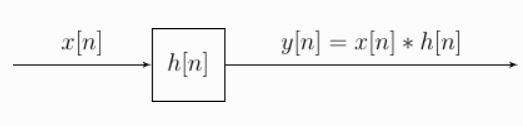
\includegraphics{Capture.jpg}
		\caption{Convolution Block Diagram}
		\label{convlution}
	\end{figure}
	The mathematical definition of convolution is:
	$$ y[n] = x[n] * h[n] = \sum_{m=-\infty}^{\infty}x[m]h[n-m] $$
	To perform discrete time linear convolotions we need to follow the following steps:
	\begin{itemize}
		\item Select the filter signal and flip the signal
		\item Pad the signal to be convolved, with zeros to sufficient lengths
		\item Align the right most element of the filter with the left most element of the signal to be convolved.
		\item Perform cross multiplication.
		\item Apply 1 unit right shift on the filter signal.
		\item Perform previous two steps until no element of the original signal is left.
	\end{itemize}
	 
	
	
	
	
	\section*{Implementation Code}  
	\captionsetup{labelformat=empty,labelsep=none}
	\lstinputlisting[style = Matlab-editor, caption={main.m}]{../lab3.m}

	\large Functions Used:
	
	\lstinputlisting[style = Matlab-editor, caption={convolution.m}]{../convolution.m}

	\lstinputlisting[style = Matlab-editor, caption={rightShift.m}]{../rightShift.m}
	\lstinputlisting[style = Matlab-editor, caption={Ws.m}]{../Ws.m}
	
	
	
\end{document}